\documentclass[11pt,a4paper]{article}

\newcommand{\tumsoTime}{09:00 น. - 12:00 น.}
\newcommand{\tumsoRound}{1}

\usepackage{../tumso}

\usepackage{soul}

\begin{document}

\begin{problem}{กระเป๋าตังดิจิตอล 2}{standard input}{standard output}{1 seconds}{256 megabytes}{100}

เนื่องด้วยรัฐบาลของประเทศแห่งหนึ่งได้ทำการหาเสียงไว้ว่าจะมีโครงการแจกเงินดิจิตอล โดยกล่าวกับประชาชนขณะหาเสียงไว้ว่า ถ้าผมจะแจกเงินพี่น้อง 1,000 บาท ประมาณตอนเที่ยง พรุ่งนี้

รัฐบาลนี้ก็ได้จัดตั้งรัฐบาลไปเป็นที่เรียบร้อย แต่ปัญหาคือไม่สามารถจัดสรรงบประมาณให้เพียงพอที่จะแจกเงินสำหรับทุกคนได้

\begin{figure}[htp]
\centering
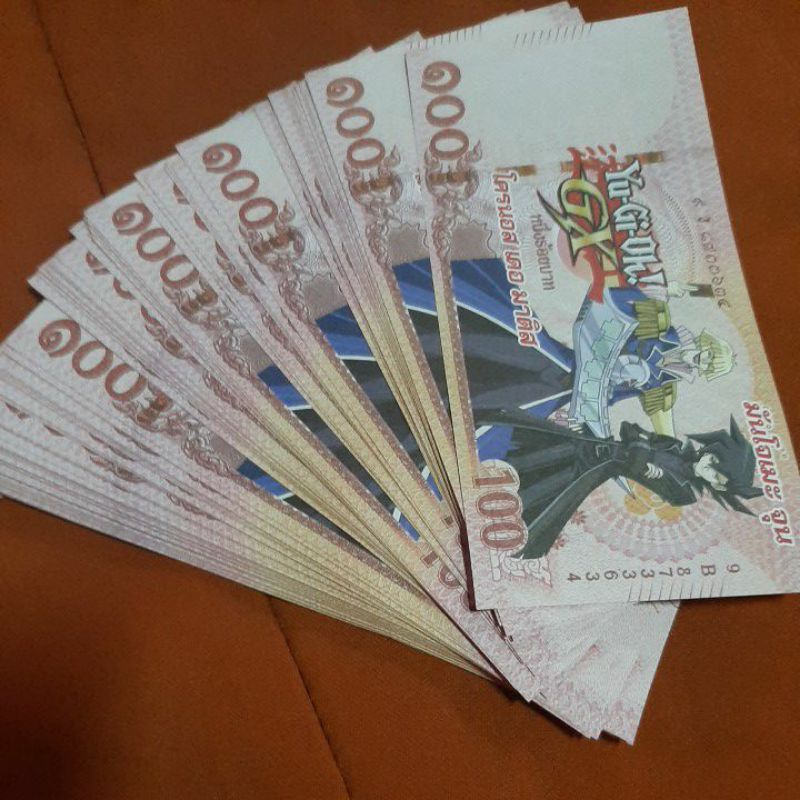
\includegraphics[width=8cm]{digitalwallet2/digitalmoney.jpeg}
\caption{เงินดิจิตอลหนึ่งพันบาทที่รัฐบาลสัญญาว่าจะแจก}
\end{figure}

รัฐบาลต้องการที่จะแจกเงินให้จำนวนน้อยที่สุด แต่หากแจกน้อยเกินไป ประชาชนจะไม่พอใจ โดยรัฐบาลคาดหวังว่าจะแจกให้ได้อย่างน้อย $T$ คน เพื่อให้ประชาชนไม่ด่าแรงมาก

เนื่องด้วยกฎเกณฑ์การแจกเงิน ต้องมีความยุติกรรม รัฐบาลจึงได้กำหนดเงื่อนไขในการแจกเงินดิจิตอลใหม่ ดังนี้

\begin{enumerate}
\item ประชาชนทุกคนมีลูกกี่คนก็ได้หรือไม่มีก็ได้ และประชาชนทุกคนจะมีบุพการีกี่คนก็ได้ (หรืออาจจะมีแต่ตายหมดแล้วก็ถือว่าไม่มี)
\item ประชาชนทุกคนที่มีรายได้เกิน $K$ บาท จะถือว่าหมดสิทธิ์
\item ประชาชนทุกคนที่มีประชาชนที่มีคุณสมบัติตามข้อ 2 เป็นบุพการีหรือลูกโดยตรง จะถือว่าหมดสิทธิ์
\end{enumerate}

รัฐบาลต้องการหาคำตอบว่า ค่า $K$ ที่น้อยที่สุดที่จะทำให้มีคนได้เงินอย่างน้อย $T$ คน เป็นเท่าไหร่

\InputFile
ข้อมูลนำเข้ามีทั้งหมด $2N+1$ บรรทัด

บรรทัดแรกประกอบด้วยจำนวนเต็ม $N$ และ $T$ แทนจำนวนคนทั้งหมด และจำนวนคนที่เป็นขั้นต่ำที่ต้องได้รับเงิน $(1 \le T \le N \le 100\,000)$

บรรทัดที่ $2i+2$ ประกอบด้วย $M_i$ แทนรายได้ของคนที่ $i$ $(0 \le i \le N - 1, 0 \le M_i \le 10^9)$

บรรทัดที่ $2i+3$ ประกอบด้วย $C, c_1, c_2, \ldots, c_C$ โดย $C$ แทนจำนวนลูกของคนที่ $i$ และ $c_k$ เป็นลูกของคนที่ $i$ $(0 \le C \le N - 1, \sum{c_k} \le 100\,000)$

\textbf{คำเตือน} อาจเกิดปรากฏการณ์โอไฮโอได้ นั่นคือลูกหลานของคน ๆ หนึ่ง อาจเป็นบรรพบุรุษของคนนั้นก็ได้ ให้ปฏิบัติตามกฎที่กำหนดไว้ แล้วจะไม่มีปัญหา

\OutputFile
ตอบจำนวนหนึ่งตัว แทน $K$ หรือคำตอบที่รัฐบาลต้องการ

\Scoring
ชุดทดสอบจะถูกแบ่งเป็น 6 ชุด จะได้คะแนนในแต่ละชุดก็ต่อเมื่อโปรแกรมให้ผลลัพธ์ถูกต้องในชุดทดสอบย่อยทั้งหมด

\begin{description}

\item[ชุดที่ 1 (15 คะแนน)] $N \le 10, M_i \le 1\,000, \sum{c_k} \le 10$

\item[ชุดที่ 2 (20 คะแนน)] $N \le 1\,000, M_i \le 1\,000, \sum{c_k} \le 10\,000$

\item[ชุดที่ 3 (15 คะแนน)] $N \le 1\,000, M_i \le 10^6, \sum{c_k} \le 10\,000$

\item[ชุดที่ 4 (15 คะแนน)] $N \le 1\,000, \sum{c_k} \le 10\,000$

\item[ชุดที่ 5 (35 คะแนน)] ไม่มีเงื่อนไขเพิ่มเติม


\end{description}

\Examples

\begin{example}
\exmp{6 3
69
2 2 3
120
2 2 3
10
0
130
1 5
999
1 5
0
0
}{130
}%
\exmp{6 6
69
2 2 3
120
2 2 3
10
0
130
1 5
999
1 5
0
0
}{999
}%
\end{example}

\Note

ตัวอย่างแรกเป็นสถานการณ์ดังนี้

\begin{itemize}
    \item มีประชาชน 6 คน ได้แก่ นายจง สีน่า $(0)$ และนาง Siuuu $(1)$ มีลูกสองคนชื่อนาย Blackslex $(2)$ และ Blueslex $(3)$ โดย Blueslex แต่งงานกับ Pinkslex $(4)$ มีลูกชื่อ Purpleslex $(5)$
    \item จง สีน่า มีรายได้ 69 บาท Siuuu มีรายได้ 120 บาท
    \item Blackslex มีรายได้ 10 บาท Blueslex มีรายได้ 130 บาท
    \item Pinkslex มีรายได้ 999 บาท และ Purpleslex ไม่มีรายได้
\end{itemize}

ตอบ 130 โดยคนที่ถูกตัดสิทธิ์คือ Pinkslex และ Purpleslex เนื่องจากผู้ปกครอง (Pinkslex) มีรายได้เกิน ทำให้มีคนได้รับสิทธิ์ 4 คน

แต่หากตอบ 120 คนที่ถูกตัดสิทธิ์คือ Pinkslex และ Purpleslex ตามด้านบน และ Blueslex จะถูกตัดสิทธิ์ ทำให้ จง สีน่า และ Siuuu ซึ่งเป็นผู้ปกครองของ Blueslex ถูกตัดสิทธิ์ตามไปด้วย คงเหลือคนที่ได้รับสิทธิ์แค่ 1 คน ซึ่งน้อยกว่าเกณฑ์ขั้นต่ำ 3 คน และจะทำให้รัฐบาลโดนด่า

\end{problem}

\end{document}
